\documentclass{amsart}
\usepackage{amsmath, amsthm, amssymb, mathtools, hyperref, tikz-cd, tikz,
tkz-graph, enumitem, nicematrix, blkarray}
\newtheorem{theorem}{Theorem}[section]
\theoremstyle{theorem}
\newtheorem{proposition}{Proposition}[section]
\theoremstyle{proposition}
\newtheorem{lemma}{Lemma}[section]
\newtheorem{corollary}{Corollary}[theorem]
\theoremstyle{remark}
\newtheorem{remark}{\underline{Remark}}[section]
\theoremstyle{definition}
\newtheorem{definition}{Definition}[section]
\theoremstyle{remark}
\newtheorem{example}{\underline{Example}}[section]
\theoremstyle{remark}
\newtheorem*{example*}{\underline{Example}}
\newcommand\sbullet[1][.5]{\mathbin{\vcenter{\hbox{\scalebox{#1}{$\bullet$}}}}}
\newcommand{\nocontentsline}[3]{}
\newcommand{\tocless}[2]{\bgroup\let\addcontentsline=\nocontentsline#1{#2}\egroup}
\newcommand{\Longupdownarrow}{\Big\Updownarrow}
\title{Higher Independence Complexes of Grid Graph $G_{n,2}$}
\author{Kumar Sannidhya SHUKLA, Prajwal UDANSHIVE}
\keywords{}
\begin{document}

\maketitle

\begin{definition}[$r$-independent set]
Let $r>0$ be an integer, and $G$ be a graph. We call a set $A\subseteq V(G)$ as $r$-\emph{independent} if each connected component of the induced subgraph $G[A]$ has at most $r$ vertices. 
\end{definition}
\begin{definition}[$r$-independence complex]
The $r$-independence complex of $G$, denoted $\operatorname{Ind}_r(G)$, is the simplicial complex whose simplices are $r$-independent sets of vertices of $G$.
\end{definition}
\begin{definition}
For $r\geq 0$, $v\in V(G)$, $S\subseteq V(G)$ is called an $r$-support of $v$ in $G$, if $v\not\in S$, $|S|=r$ and $G[S\cup v]$ is a connected graph. Let $\operatorname{Supp}_{r}(v,G)$ denote the collection of all $r$-supports in $G$. We say that $\operatorname{Supp}_r(v,G)$ is connected if the induced subgraph $G[S]$ is connected for all $r$-supports $S$ of $v$.
\end{definition}
\begin{theorem}
Let $G$ be a connected graph, $v\in V(G)$ and $\operatorname{Supp}_r(v,G) = \{S_1,\dots,S_n\}$. If $\operatorname{Supp}_r(v,G)$ is connected and $N(v)\subseteq N[S_i]$ for each $i\in[n]$, then
\begin{equation*}
\operatorname{Ind}_r(G) = \bigvee\limits_{i=1}^{n}\Sigma^r(\operatorname{Ind}_r(G-N[S_i])).
\end{equation*}
\end{theorem}
As an illustration, we work with grid graphs $G_{2,n}$.
\begin{center}
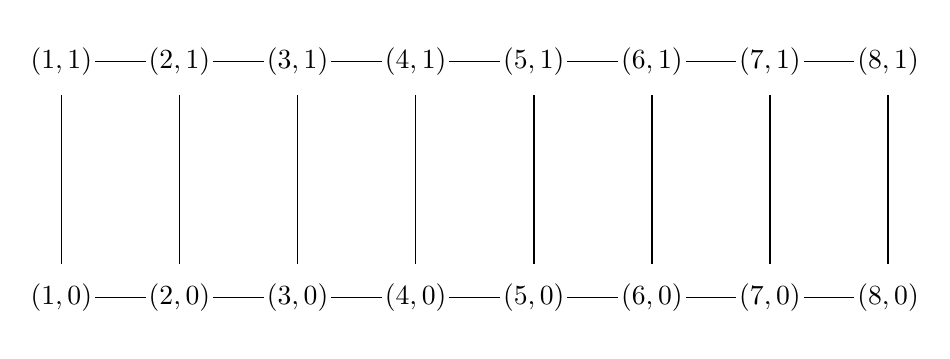
\begin{tikzpicture}
  \tikzset{VertexStyle/.style = {shape = circle,minimum size = 2pt,inner sep=0pt}}
\Vertex[style={minimum size=0.01cm,shape=circle},LabelOut=false,L=\hbox{$(1, 1)$},x=0.0cm,y=3.0cm]{v0}
\Vertex[style={minimum size=0.1cm,shape=circle},LabelOut=false,L=\hbox{$(2, 1)$},x=1.5cm,y=3.0cm]{v1}
\Vertex[style={minimum size=0.1cm,shape=circle},LabelOut=false,L=\hbox{$(3, 1)$},x=3.0cm,y=3.0cm]{v2}
\Vertex[style={minimum size=0.1cm,shape=circle},LabelOut=false,L=\hbox{$(4, 1)$},x=4.5cm,y=3.0cm]{v3}
\Vertex[style={minimum size=0.1cm,shape=circle},LabelOut=false,L=\hbox{$(5, 1)$},x=6.0cm,y=3.0cm]{v4}
\Vertex[style={minimum size=0.1cm,shape=circle},LabelOut=false,L=\hbox{$(6, 1)$},x=7.5cm,y=3.0cm]{v5}
\Vertex[style={minimum size=0.1cm,shape=circle},LabelOut=false,L=\hbox{$(7, 1)$},x=9.0cm,y=3.0cm]{v6}
\Vertex[style={minimum size=0.1cm,shape=circle},LabelOut=false,L=\hbox{$(8, 1)$},x=10.5cm,y=3.0cm]{v7}
\Vertex[style={minimum size=0.1cm,shape=circle},LabelOut=false,L=\hbox{$(1, 0)$},x=0.0cm,y=0.0cm]{v8}
\Vertex[style={minimum size=0.1cm,shape=circle},LabelOut=false,L=\hbox{$(2, 0)$},x=1.5cm,y=0.0cm]{v9}
\Vertex[style={minimum size=0.1cm,shape=circle},LabelOut=false,L=\hbox{$(3,0)$},x=3.0cm,y=0.0cm]{v10}
\Vertex[style={minimum size=0.1cm,,shape=circle},LabelOut=false,L=\hbox{$(4, 0)$},x=4.5cm,y=0.0cm]{v11}
\Vertex[style={minimum size=0.1cm,shape=circle},LabelOut=false,L=\hbox{$(5, 0)$},x=6.0cm,y=0.0cm]{v12}
\Vertex[style={minimum size=0.1cm,shape=circle},LabelOut=false,L=\hbox{$(6, 0)$},x=7.5cm,y=0.0cm]{v13}
\Vertex[style={minimum size=0.1cm,shape=circle},LabelOut=false,L=\hbox{$(7, 0)$},x=9.0cm,y=0.0cm]{v14}
\Vertex[style={minimum size=0.1cm,shape=circle},LabelOut=false,L=\hbox{$(8, 0)$},x=10.5cm,y=0.0cm]{v15}
%
\Edge[lw=0.02cm,style={color=black,},](v0)(v1)
\Edge[lw=0.02cm,style={color=black,},](v0)(v8)
\Edge[lw=0.02cm,style={color=black,},](v1)(v2)
\Edge[lw=0.02cm,style={color=black,},](v1)(v9)
\Edge[lw=0.02cm,style={color=black,},](v2)(v3)
\Edge[lw=0.02cm,style={color=black,},](v2)(v10)
\Edge[lw=0.02cm,style={color=black,},](v3)(v4)
\Edge[lw=0.02cm,style={color=black,},](v3)(v11)
\Edge[lw=0.02cm,style={color=black,},](v4)(v5)
\Edge[lw=0.02cm,style={color=black,},](v4)(v12)
\Edge[lw=0.02cm,style={color=black,},](v5)(v6)
\Edge[lw=0.02cm,style={color=black,},](v5)(v13)
\Edge[lw=0.02cm,style={color=black,},](v6)(v7)
\Edge[lw=0.02cm,style={color=black,},](v6)(v14)
\Edge[lw=0.02cm,style={color=black,},](v7)(v15)
\Edge[lw=0.02cm,style={color=black,},](v8)(v9)
\Edge[lw=0.02cm,style={color=black,},](v9)(v10)
\Edge[lw=0.02cm,style={color=black,},](v10)(v11)
\Edge[lw=0.02cm,style={color=black,},](v11)(v12)
\Edge[lw=0.02cm,style={color=black,},](v12)(v13)
\Edge[lw=0.02cm,style={color=black,},](v13)(v14)
\Edge[lw=0.02cm,style={color=black,},](v14)(v15)
\end{tikzpicture}
\end{center}
\begin{corollary} 
$\operatorname{Ind}_{n-1}(G_{2,n})$ is contractible for $n\geq 4$.
\end{corollary}
\begin{proof} Label $G_{2,n}$ per the above illustration. Let $S$ be an $(n-1)$-support of $v=(1,0)$. The edge(s) connecting $v$ to $G[S]$ are precisely $\{v,(1,1)\}$ or $\{v,(2,0)\}$, and hence are the only new edge(s) introduced to $G[S]$ when we adjoin $v$. Since $G[S\cup v]$ is connected, removal of $v$ cannot disconnect $G[S]$. Hence, $S$ must contain either $(1,1)$ or $(2,0)$, which proves $N[v]\subseteq N[S]$.
\par Let $S=\{(x_i,y_i)\mid1\leq i\leq n-1\}$. Let $c = \max\limits_{1\leq i\leq n-1}x_i$. Since $(1,0)\not\in S$, notice that $2c>n-1$, as $\{(x,y)\mid 1\leq x\leq c,\,\,y=0,1\}$ properly contains $S$. Therefore,
\begin{equation}
c\geq \Bigl\lfloor\frac{n}{2}\Bigl\rfloor
\end{equation}
Let $d = |V(G-N[S])|$. As $N[S]$ must contain $(c+1,0)$ or $(c+1,1)$, $d<2(\lfloor\frac{n}{2}\rfloor-1)$. But then, $\operatorname{Ind}_{n-1}(G-N[S])$ is a $d$-simplex, and hence must be contractible. We are now done by the earlier theorem.
\end{proof}
\begin{remark}
For $n=3$, $S = \{\}$
\end{remark}
\begin{remark}
Recall: Devadoss \cite{dev} defined a similar notion of \emph{tube}: A \emph{tube} $S$ is a set $\varnothing\neq S\subsetneq V(G)$ with $G[S]$ connected. 
\end{remark}
\end{document}
